\documentclass[a4paper,
12pt,
headings=small,
bibliography=totoc,
%toc=flat, % toc=graduated -> linksbündig
%toc=listof,     % Abbildungs-, Tabellenverzeichnis
toc=index,      % Stichwortverzeichnis
ngerman,
final           % Status final/draft
]{scrreprt}

%listof=totoc,
%index=totoc,

% bibliography=totoc, index=totoc, listof=totoc
                % verzeichnisse ins TOC
% toc=flat      % wenn zu /tiefe/ Punkte im TOC entstehen -> quasi-tabellarisches TOC
% toc=listof    % Abb- und Tabellenverzeichnis stehen im TOC, nicht nummeriert
% toc=idx       % Stichwortverzeichnis wird ins TOC aufgenommen, nicht nummeriert

% einige Teile/Snippets von <http://blog.stefan-macke.com/2007/10/30/neue-version-meiner-latex-vorlage-fuer-die-diplomarbeit-an-der-fhwt/> übernommen


% sysconfig und pakete
\usepackage[ngerman]{babel}
\usepackage[utf8]{inputenc}
\usepackage{graphicx}                   	%
\usepackage{tikz}					        % tikz-grafiken
\usetikzlibrary{shapes.multipart,trees,arrows,shapes,fit,backgrounds,topaths,positioning,fadings,decorations,automata}
\usepackage{pgfbaselayers}                  % GFX-Layer
\usepackage{eurosym}                    	% \euro Währungszeichen
\usepackage{geometry}                   	% Einfache Definition der Zeilenabstände, Seitenränder etc.
\usepackage{setspace}
\usepackage{todonotes}                  	% \todo{} Anmerkungen
\usepackage[binary]{SIunits}			% \mega\byte -- http://www.ctan.org/tex-archive/macros/latex/contrib/SIunits/
\usepackage{varioref}			% automatische Seiten-referenz etc.
\usepackage{url}
\usepackage{appendix}
\usepackage{paralist}           % Inline-Listen
\usepackage{tabularx}           % variabel/feste Tabellen-Spalten
\usepackage{booktabs}			% tabular-stuff

%% header/footer
\usepackage[nouppercase,                % nicht komplett in Großbuchstaben
    automark,                           % Kapitelangaben in Kopfzeile automatisch erstellen
    headsepline,                        % Trennlinie unter Kopfzeile
    ilines                              % Trennlinie linksbündig ausrichten
    ]{scrpage2}


\usepackage[acronym,			% new glossary with acronyms
    toc,				% add to TOC
    numberline,         % add page-number in TOC
    %style=listdotted,			% glossaries.pdf, page 55
    style=list,			% glossaries.pdf, page 55
    %header=plain,
    %cols=3,
    footnote,				% create footnote on new-acronym
    %toctitle={},
    numberedsection,
    section=chapter
]{glossaries}        % Glossar und Abkürzungen
\usepackage{makeidx}                    % Index-Ausgabe mit \printindex

% Symbolverzeichnis ------------------------------------------------------------
%   Symbolverzeichnisse bequem erstellen. Beruht auf MakeIndex:
%     makeindex.exe %Name%.nlo -s nomencl.ist -o %Name%.nls
%   erzeugt dann das Verzeichnis. Dieser Befehl kann z.B. im TeXnicCenter
%   als Postprozessor eingetragen werden, damit er nicht st�ndig manuell
%   ausgef�hrt werden muss.
%   Die Definitionen sind ausgegliedert in die Datei "Glossar.tex".
% ------------------------------------------------------------------------------
\usepackage[intoc]{nomencl}
\let\abbrev\nomenclature
\renewcommand{\nomname}{Abkürzungsverzeichnis}
\setlength{\nomlabelwidth}{.25\hsize}
\renewcommand{\nomlabel}[1]{#1 \dotfill}
\setlength{\nomitemsep}{-\parsep}

% Zum Einbinden von Quellcode
\usepackage{listings}
\usepackage{xcolor}
\definecolor{hellgelb}{rgb}{1,1,0.9}
\definecolor{colKeys}{rgb}{0,0,1}
\definecolor{colIdentifier}{rgb}{0,0,0}
\definecolor{colComments}{rgb}{1,0,0}
\definecolor{colString}{rgb}{0,0.5,0}
\lstset{%
    float=hbp,%
    basicstyle=\texttt\small, %
    identifierstyle=\color{colIdentifier}, %
    keywordstyle=\color{colKeys}, %
    stringstyle=\color{colString}, %
    commentstyle=\color{colComments}, %
    columns=flexible, %
    tabsize=2, %
    frame=single, %
    extendedchars=true, %
    showspaces=false, %
    showstringspaces=false, %
    numbers=left, %
    numberstyle=\tiny, %
    breaklines=true, %
    backgroundcolor=\color{hellgelb}, %
    breakautoindent=true, %
    escapeinside={(*@}{@*)}% use (*@\label{comment}@*)
%    captionpos=b%
}



% Wichtig für korrekte Zitierweise, use bibtex-style dinat
\usepackage{natbib}
\usepackage[chapter,numbib,numindex,notlof]{tocbibind}
% Quellenangaben in eckige Klammern fassen
%\bibpunct{[}{]}{;}{a}{}{,~}


\usepackage[colorlinks,			% Links farbig hervorheben
%    breaklinks,					% Links umbrechen, passiert automatisch bei nutzung von pdftex
    bookmarks,					%
    hyperindex=false,
    % uncomment the following line if you want to have black links (e.g., for printing)
    urlcolor=black, linkcolor=black, citecolor=black, %pagecolor=Black,%
    pdfauthor={Oluf Lorenzen},
    pdftitle={Split-Access-Routing mit Priorisierung auf Linux-Basis},
    pdfkeywords={Linux,Debian,routing}]{hyperref}
                                        % PDF-Gefrickel
                                        % Lange URLs umbrechen ...
%\usepackage{breakurl}

\usepackage{courier}

% debugging etc.
\usepackage[l2tabu, orthodox, abort]{nag}


%%% Index-, Abkürzungsverzeichnis und Gloassar erstellen und einbinden
\makeindex
%\makenomenclature
\makeglossary


%%% Kopf- und Fußzeilen, Seitenränder etc.

% Kopf- und Fußzeilen
\pagestyle{scrheadings}

% löscht voreingestellte Stile
\clearscrheadings
\clearscrplain


%%% Schusterjungen/Hurenkinder
\clubpenalty = 10000 % schliesst Schusterjungen aus
\widowpenalty = 10000 % schliesst Hurenkinder aus
\displaywidowpenalty = 10000 % und nochmal für Formeln


%%% Zeilenabstand auf 1.5-Zeilig
\onehalfspacing

%%% Seitenränder
%\geometry{paper=a4paper,left=30mm,right=40mm,top=10mm,bottom=65mm}
\geometry{paper=a4paper,left=25mm,right=20mm,top=25mm,bottom=30mm}
                                % Vorgabe der IHK Hannover, 2009


% Kopf- und Fußzeile auch auf Kapitelanfangsseiten
\renewcommand*{\chapterpagestyle}{scrheadings}

% Schriftform der Kopfzeile
%\renewcommand{\headfont}{%
%\normalfont
%}

% Kopfzeile
\ohead{\titel}
%\ihead{\large{\textsc{\titel}}\\    \small{\untertitel} \\[2ex] \textit{\headmark}}
%\chead{}
%\ohead{\includegraphics[scale=0.4]{FHWTLogoKlein.jpg}}
%%
%\setlength{\headheight}{21mm} % Höhe der Kopfzeile
%\setheadwidth[0pt]{textwithmarginpar} % Kopfzeile über den Text hinaus verbreitern
%\setheadsepline[text]{0.4pt} % Trennlinie unter Kopfzeile

% Fußzeile
\ifoot{\autor}
\cfoot{}
\ofoot{\pagemark}


% erzeugt ein wenig mehr Platz hinter einem Punkt
\frenchspacing


% Quellcode-Ausgabe formatieren
\lstset{numbers=left, numberstyle=\tiny, numbersep=5pt, breaklines=true}
\lstset{emph={square}, emphstyle=\color{red}, emph={[2]root,base}, emphstyle={[2]\color{blue}}}

% Fußnoten fortlaufend durchnummerieren

\KOMAoption{listof}{numberedtotoc}


% Informationen ------------------------------------------------------------
%   Definition von globalen Parametern, die im gesamten Dokument verwendet
%   werden k�nnen (z.B auf dem Deckblatt etc.).
% --------------------------------------------------------------------------
\newcommand{\titel}{Split-Access-Routing mit Priorisierung auf Linux-Basis}
\newcommand{\untertitel}{Dokumentation der betrieblichen Projektarbeit}
\newcommand{\autor}{Oluf Lorenzen}
\newcommand{\auftraggeber}{axxeo GmbH}
\newcommand{\jahr}{2009}

% Eigene Befehle und typographische Auszeichnungen f�r diese
\newcommand{\AutorZ}[1]{\textsc{#1}}
\newcommand{\Autor}[1]{\AutorZ{\citeauthor{#1}}}

\newcommand{\NeuerBegriff}[1]{\textbf{#1}}

\newcommand{\Fachbegriff}[1]{\textit{#1}}
\newcommand{\Prozess}[1]{\textit{#1}}
\newcommand{\Webservice}[1]{\textit{#1}}

\newcommand{\Eingabe}[1]{\texttt{#1}}
\newcommand{\Code}[1]{\texttt{#1}}
\newcommand{\Datei}[1]{\texttt{#1}}

\newcommand{\Datentyp}[1]{\textsf{#1}}
\newcommand{\XMLElement}[1]{\textsf{#1}}

\newcommand{\std}{\hour}
%\newcommand{\min}{\minute}

\let\textquotedbl="

\newcommand{\gt}{\textgreater}
\renewcommand{\le}{\textless}
\newcommand{\tq}{\textquotedbl}

% Abk�rzungen mit korrektem Leerraum
\newcommand{\sog}{\mbox{sog.\ }}
\newcommand{\bzw}{\mbox{bzw.\ }}
\newcommand{\vgl}{\mbox{Vgl.\ }}
\newcommand{\ua}{\mbox{u.\,a.\ }}
\newcommand{\oae}{\mbox{o.\,ä.\ }}
\newcommand{\zB}{\mbox{z.\,B.\ }}
\newcommand{\ca}{\mbox{ca.\ }}
\newcommand{\etc}{\mbox{etc.\ }}
\newcommand{\bs}{$\backslash$}



\begin{document}
\begin{titlepage}
\titlehead{{\Large \auftraggeber\\}
  Kniestraße 27\\
  30167 Hannover}
\subject{\untertitel}
\date{Oktober 2009}
\title{\titel}
\author{\autor}
\publishers{betreut durch Dipl.-Inform. Andreas Godzina\\\vspace{2cm}Ausbildungsberuf: Fachinformatiker Systemintegration\\Durchführungszeitraum: 12.10.2009 -- 20.10.2009}

\maketitle

\end{titlepage}

\pagenumbering{Roman}
\tableofcontents % Inhaltsverzeichnis


% Abkürzungsverzeichnis
\newglossaryentry{fingerprint}{name=Fingerprint,description={engl. für Fingerabdruck}}
\newglossaryentry{Debian}{name=Debian,description={Linux-Distribution}}
\newglossaryentry{routing-pol-db}{name=routing policy database
,description={engl., Datenbank für Routing-Festlegungen}}
\newglossaryentry{tc}{name=tc(8),description={Tool zur Kontrolle des Netzwerkverkehrs im Linux-Kernel}}
\newglossaryentry{tcng}{name=tcng(1),description={Tool zur Kompilierung von Scripten in tc-Befehle}}
\newglossaryentry{egress}{name=egress,description={engl. für Ausgehend}}
\newglossaryentry{ingress}{name=ingress,description={engl. für Eingehend}}
\newglossaryentry{qdisc}{name=qdisc,description={Scheduler (regelt die zeitliche Ausführung mehrerer Prozesse) -- der Standard-Scheduler für Linux-Netzwerkinterfaces ist FIFO}}
\newglossaryentry{bucket}{name=bucket,description={engl. für Eimer}}
\newglossaryentry{token}{name=token,description={engl. für Jeton, Wertmarke, {\oae}}}
\newglossaryentry{hping}{name=hping,description={Tool um Netzwerkpakete zu erzeugen}}
\newglossaryentry{Routing}{name=Routing,description={Funktion um Wege bei der Nachrichtenübermittlung festzulegen}}
\newglossaryentry{Cache}{name=Cache,description={Zwischenspeicher}}
\newglossaryentry{Policy}{name=Policy,description={engl. für Richtlinie}}


\newacronym{IP}{IP}{Internet Protocol}
\newacronym{ssh}{SSH}{Secure Shell, sicherer Ersatz für \emph{telnet}}
\newacronym{isp}{ISP}{Internet Service Provider / Internetdienstanbieter}
\newacronym{sar}{S-A-R}{Split-Access-Routing, Internetzugang über mehrere Anbindungen gleichzeitig}
\newacronym{ADSL}{ADSL}{Asymmetric Digital Subscriber Line}
\newacronym{SDSL}{SDSL}{Symmetric Digital Subscriber Line}
\newacronym{VDSL2+}{VDSL2+}{Extended bandwidth Asymmetric Digital Subscriber Line 2}
\newacronym{TBF}{TBF}{Token Bucket Filter -- Scheduler, welcher die durchschnittliche Datenrate begrenzt}
\newacronym{HTB}{HTB}{\href{http://luxik.cdi.cz/~devik/qos/htb/}{Hierarchical Token Bucket packet scheduler} -- eine Variante des \emph{Token-Bucket-Filter}}
\newacronym{FIFO}{FIFO}{First-In-First-Out -- Verfahren, wie Daten abgearbeitet werden ({\vgl} Schlange)}
\newacronym{NAT}{NAT}{Network-Address-Translation, umsetzung von Netzwerkadressen}
\newacronym{VoIP}{VoIP}{Voice over Internet Protocol, Internet-Telefonie}
\newacronym{NIC}{NIC}{Network Interface - Netzwerkkarte}
\newacronym{SMTP}{SMTP}{Simple Mail Transfer Protocol, Netzwerkprotokoll zur Übertragung von E-Mails}
\newacronym{HTTP}{HTTP}{Hypertext Transfer Protocol, Netzwerkprotokoll zur Übertragung von Webseiten}





\nomenclature{API}{Application Programming Interface}
\nomenclature{ARIS}{Architektur integrierter Informationssysteme}
\nomenclature{BPR}{Business Process Reengineering}
\nomenclature{eEPK}{erweiterte Ereignisgesteuerte Prozesskette}
\nomenclature{EPK}{Ereignisgesteuerte Prozesskette}
\nomenclature{JMS}{Java Message Service}
\nomenclature{SDK}{Software Development Kit}
\nomenclature{URI}{Uniform Resource Identifier}
\nomenclature{URL}{Uniform Resource Locator}
\nomenclature{URN}{Uniform Resource Name}
\nomenclature{W3C}{World Wide Web Consortium}
\nomenclature{XML}{Extensible Markup Language}
\nomenclature{XPath}{XML Path Language}
\nomenclature{XSL}{Extensible Stylesheet Language}
\nomenclature{XSLT}{XSL Transformations}



% arabische Seitenzahlen im Hauptteil
\clearpage
\pagenumbering{arabic}

\chapter{Einleitung}
\section{Umfeld der Installation und Ist-Zustand}
Die {\auftraggeber} ist als Linux- und Netzwerkdienstleister 2004 in Hannover gegründet worden. Der Kerndienstleistungsbereich umfasst größtenteils \textit{second-} und \textit{third-Level}-Support an \gls{Debian}-Linux-Servern, Planung und Bereitstellung von Firewall- und Serversystemen sowie deren Wartung.
Das Projekt "`\textit{\titel}"' ist ein In-House-Projekt, welches nach erfogreicher Implementierung im Produktivnetz unter anderem für Schulungszwecke und zum Sammeln von Erfahrung eingesetzt werden soll. Darüber hinaus wird nach einiger Zeit die Funktionalität auch in eigene Produkte übernommen.
\subsection*{Beschreibung Ist-Zustand}
Derzeit ist die {\auftraggeber} über einen einzelnen \gls{isp} mit 2000~{\kibi\bit\per\second} an das Internet angebunden (Siehe Abb. \vref{fig:netzplan}, "`alte Verbindung"').
Diese Leitung wird firmenintern von drei bis vier Personen und innerhalb eines untervermieteten Büros von weiteren zwei bis drei Personen genutzt. Außerdem wird die Leitung zur Anbindung eines Mailservers und zum Download nächtlicher, inkrementeller Backups von Kundenservern genutzt. Für die tägliche Arbeit ist seitens der {\auftraggeber} der Zugriff via \gls{ssh} auf entfernte Maschinen, sowie die Nutzung der Protokolle \gls{HTTP} und \gls{SMTP} essentiell.

Durch die Untervermietung hat sich die Auslastung der Internetleitung geändert. So war zuvor selten eine höhrere Latenz durch starke Auslastung festzustellen -- nun ist eine volle Auslastung häufig gegeben, was die Support-Arbeit via \gls{ssh} stark erschwert und verlangsamt.

\section{Beschreibung Soll-Zustand}
Um die Bandbreite zu priorisieren und die Last generell auf eine zweite Leitung aufzuteilen, wurde zunächst das Tool \gls{tc} und das LARTC-Howto \citep{LARTC} zur Problemlösung favorisiert. Diese Vorauswahl basiert auf einer generellen Präferenz der {\auftraggeber} für Lösungen, die sich mit \gls{Debian}-Bordmitteln und nach \gls{Debian}-Regeln erreichen lassen. Die Arbeit via SSH muss troz hoher Auslastung der Bandbreite latenzfrei möglich sein.
\section{Zeitplanung}
\begin{table}[htb]
\centering
\begin{tabular}{p{12cm}|l}
geplante Tätigkeit & geplante Dauer\\\toprule
Basiskonzept, Information, \etc & 3-4 \std\\\hline
Installation, Konfiguration, Einbinden in bestehende Scripte & 5 \std\\\hline
Anpassung von Parametern in Absprache mit Auftraggeber & 1 \std\\\hline
Test des Aufbaus, Zusammenspiel von vorhandenen Systemscripten mit neuer Konfiguration bei Reboot, Anpassung \etc & 4 \std\\\hline
Erstellung von Scripten um Leitungs-Ausfall festzustellen & 3 \std\\\hline
Laufzeit-Tests (Last-Verteilung, Priorisierung), Simulation von versch. Ausfällen (Netzwerk-Interface, Next-Hop-Router, ...) & 7 \std\\\hline
Dokumentation & 8 \std\\\hline
variable Pufferzeit & 3 \std
\end{tabular}
\caption{Planung der benötigten Zeit innerhalb des vorgeschriebenen Zeitrahmens von 35 \std}
\label{tab:zeit-geplant}
\end{table}

\chapter{Planung}
Es wurde zunächst ein Netzplan erstellt (Abb. \vref{fig:netzplan}), der der besseren Übersicht und Darstellbarkeit halber ab dem ersten Router nach \texttt{fire\-wall.office.axxeo.de} stark vereinfacht und auf einen weiteren Hop beschränkt ist. In der Realität folgen nach \texttt{Router eins} und \texttt{Router zwei} noch weitere Hops.
Für alle Netze außerhalb von \texttt{firewall.office.{$_{\hookleftarrow}$}\\axxeo.de} wurden private Netzbereiche gewählt, um nicht mit bereits vergebenen, öffentlichen \gls{IP}-Adressen in Berührung zu kommen.

\input{Inhalt/Grafiken/netzplan}

\section{Ressourcenplanung}
Für die Umsetzung des Projekts sind keine Anschaffungen oder speziellen Einplanungen nötig; die vorhandene Firewall \texttt{firewall.office.axxeo.de} (Abb. \vref{fig:netzplan}) wird erweitert und für Simulationen steht eine gemeinsam genutzte VMWare-Workstation bereit. Zur Erarbeitung wird ein bereits zugewiesener Standard-PC-Arbeitsplatz verwendet.

\section{Split-Access-Routing}
Um als ersten Schritt ein überhaupt laufendes Setup mit \gls{sar} zu erzeugen, wurde der im LARTC beschriebene Aufbau übernommen und den Umständen angepasst:

\begin{enumerate}
 \item Erstellen von einer \gls{Routing}-Tabelle für jedes externe Interface:\\
    \texttt{echo -e {\tq}200 one{\bs}n 201 two{\tq} {\gt}{\gt} /etc/iproute2/rt\_table}
 \item Hinzufügen von zwei Regeln in die \gls{Routing}-\gls{Policy}-Datenbank, um Antworten auf Anfragen aus den jeweils anliegenden Netzbereichen (10.1.0.0/24 und 10.2.0.0/24) auch wieder auf dem passenden Interface zu versenden:\\
    \texttt{ip rule add from 10.1.0.0/24 table one\\ip rule add from 10.2.0.0/24 table two}
 \item Hinzufügen von Routen in die im ersten Schritt erstellten Tabellen; ohne diese Einträge würden die im zweiten Schritt aufgegriffenen Pakete die jeweilige Routing-Tabelle durchlaufen, auf keinen Eintrag passen und dann wieder die main-Tabelle passieren:\\
    \texttt{ip r r 127.0.0.0/8 dev lo table one\\ip r r 10.2.0.0/24 dev eth2 src 10.2.0.1 table one\\ip r r default dev eth1 table one\\
	ip r r 127.0.0.0/8 dev lo table one\\ip r r 10.1.0.0/24 dev eth1 src 10.1.0.1 table two\\ip r r default dev eth2 table two}
 \item Ersetzen der default-Route mit einem eins-zu-eins-Balancing:\\
    \texttt{ip r r default scope global nexthop via 10.1.0.2{$_{\hookleftarrow}$}\\ {$^{\hookrightarrow}$}dev eth1 weight 1 nexthop via 10.2.0.2 dev eth2 weight 1}
\end{enumerate}

\section{Priorisierung}
Zum Verständnis von Priorisierung und Traffic-Shaping generell wurde wieder das LARTC \citep{LARTC} genutzt. Nach der Lektüre des Kapitels 9 war ersichtlich, wie die Priorisierung funktioniert und, dass die Syntax von \gls{tc} selbst weder leicht zu verstehen, noch leicht zu schreiben ist. Nach weiterer Recherche\footnote{{\ua}\url{http://tldp.org/HOWTO/HOWTO-INDEX/networking.html}} wurde ein Howto für das Tool \gls{tcng} \citep{TCNGHTB} gefunden.
Auch hier wurde nah am Beispiel gearbeitet und die Konfiguration nur wenig verändert. Die \gls{tcng}-Scripte für die Schnittstellen eth1 und eth2 auf \texttt{firewall.office.axxeo.de} sind unter \vref{lst:eth1_tcc} und \vref{lst:eth2_tcc} Angehängt.

Die Einteilung der Bandbreite für jedes Interface hat sich dabei folgendermaßen ergeben:
An eth1 steht die \gls{SDSL}-Leitung mit 2000/2000~{\kibi\bit\per\second} (Zeile \vref{lst:eth1.tcc.eth1-speed}) zur Verfügung, über welche Fernwartung via SSH erfolgen muss, da nur die auf diesem Interface liegende IP auf den Maschinen der Kunden freigeschaltet ist. An eth2 steht eine \gls{VDSL2+}-Leitung mit 50000/10000~{\kibi\bit\per\second} (Zeile \vref{lst:eth2.tcc.eth2-speed}) zur Verfügung, welche von einem weiteren Mieter im Hause betrieben wird und auf Fair-Use-Basis genutzt werden kann.

Der Aufbau der \gls{tcng}-Scripte ist hierarchisch und recht einfach; erklärt wird folgend der Aufbau des Scripts für eth1.

Als erstes wird das Interface definiert (Zeile \vref{lst:eth1.tcc.eth1}), für das \gls{tc}-Regeln erstellt werden sollen, danach wird die \gls{egress}- oder \gls{ingress}-\gls{qdisc} gewählt (Zeile \ref{lst:eth1.tcc.egress}), in der wiederum Definitionen für Traffic-Gruppen (Zeile \ref{lst:eth1.tcc.interactive-out}, \ref{lst:eth1.tcc.interactive-in}, \ref{lst:eth1.tcc.other}) und die darauf angewendeten Regeln definiert werden (Zeile \ref{lst:eth1.tcc.interactive-out-rate}, \ref{lst:eth1.tcc.interactive-in-rate}, \ref{lst:eth1.tcc.other-rate}). Verwendet wird allerdings nur die \gls{egress}-\gls{qdisc}, da nur die Datenströme wirklich beeinflusst werden können, die von der Maschine selber ausgehen.
Für alle Datenströme, die möglichst ohne Verzögerung übertragen werden sollen, sind die Klassen \emph{\$interactive\_*}  vorgesehen (Zeile \ref{lst:eth1.tcc.interactive-out-rate}, \ref{lst:eth1.tcc.interactive-in-rate}). % Ob diese Liste an Kriterien im Echtbetrieb auch wirklich den Traffic erfasst, den man hoch priorisieren will, muss noch überprüft werden\todo{umschreiben}.
Alle anderen Datenströme werden über die Klasse \emph{\$other} (Zeile \ref{lst:eth1.tcc.other}) abgewickelt.

Alle Regeln sind innerhalb des \gls{HTB} (Zeile \ref{lst:eth1.tcc.htb}) definiert. Mit der Wahl des \gls{HTB} wird versucht, einen einfachen, durchschaubaren\footnote{"`As said before, CBQ is the most complex qdisc available, the most hyped, the least understood, and probably the trickiest one to get right"' \citep[Kapitel 9.5.4.]{LARTC}} Einstieg zu finden, der laut Entwickler auch genau zum Anwendungsfall passt\footnote{"`One requirement for link-sharing is to share bandwidth on a link between multiple organizations, where each organization wants to receive a guaranteed share of the link bandwidth during  congestion, but where bandwidth that is not being used by one  organization should be available to other organizations sharing  the link."' \citep[Kapitel 2.8]{DSERV}}.
Generell erlaubt der hierarchische Aufbau eine feingranulare Aufteilung der Bandbreite nach vielen Parametern.

Für ein besseres Verständnis ist der implementierte Aufbau unter Abb. \vref{abb:tcc-tree-eth1} auch als Grafik zu sehen.

\section*{Detail-Analyse der tcng-Scripte (Listing \vref{lst:eth1_tcc} und \vref{lst:eth2_tcc})}
Die folgenden Ausführungen wurde zu einem gewissen Teil von docum.org \citep{DOCUMHTB} übersetzt, da die Formulierungen sehr treffend sind.
\begin{description}
  \item[rate] die garantierte Bandbreite einer Klasse
  \item[ceil] die maximale Bandbreite, die eine Klasse nutzen kann
\end{description}

Den Parametern \emph{rate}/\emph{burst} und \emph{ceil}/\emph{cburst} werden {\sog}\emph{\gls{token} \glspl{bucket}} zugewiesen. Der \emph{rate-bucket} wird mit \gls{token} und der \emph{ceil-bucket} mit \emph{c}\gls{token} gefüllt - es gibt also für jede Klasse zwei \glspl{bucket}. Die Geschwindigkeit mit der die Tolken gefüllt werden wird über burst und cburst festgelegt.


Ein Beispiel mit \emph{rate}=100~{\byte\per\second}, \emph{burst}=300~{\byte} und einem Datenversand von 200~{\byte\per\second}:
\begin{figure}[htb]
  \centering
  \includegraphics[height=5.5cm]{Inhalt/Grafiken/bandbreite-gewuenscht.png}
  % null.png: 1030x633 pixel, 120dpi, 21.80x13.40 cm, bb=0 0 618 380
  \caption{gewünschte Bandbreite}
  \label{fig:bandbreite-gewuenscht}
\end{figure}

\begin{figure}[htb]
  \centering
  \includegraphics[height=5.5cm]{Inhalt/Grafiken/bandbreite-nach-htb.png}
  % null.png: 1030x633 pixel, 120dpi, 21.80x13.40 cm, bb=0 0 618 380
  \caption{Bandbreite nach HTB}
  \label{fig:bandbreite-nach-htb}
\end{figure}

\begin{itemize}
  \item\textbf{0 - 3~Sekunden:} Datenversand kann in voller Geschwindigkeit erfolgen, es werden nachlaufende token und token aus dem bucket genutzt
  \item\textbf{4 - \dots~Sekunden:} bucket ist leer, es werden nachlaufende token genutzt
\end{itemize}


%Der rate-Wert bedeutet nun, dass der Rate-Bucket mit 100 token{\per\second} gefüllt wird bis er voll ist (100 token, burst). Alle weiteren token für diesen bucket werden an den ceil-bucket weitergegeben bis dieser auch gefüllt ist (300 ctoken, cburst).
%Sobald auch dieser bucket gefüllt ist, werden die token verworfen.

%Jeder token repräsentiert ein Byte - wenn also 100 Byte versandt werden sollen, werden 100 token benötigt. Beide Token werden gleich stark belastet.

%\input{Inhalt/Grafiken/token-detail}

%Es wird davon ausgegangen, dass alle Buckets gefüllt sind, da die Leitung davor nicht genutzt wurde.
%\begin{itemize}
%  \item\textbf{0 - 3~Sekunden:} der \emph{rate}-\gls{bucket} wird mit 100~token{\per\second} gefüllt und der \emph{ceil}-\gls{bucket} ist 300 ctoken groß.\\Es werden insgesamt 200~token{\per\second} genutzt, also können die überschüssigen 100~token{\per\second} in den ersten drei Sekunden aus dem \emph{ceil}-\gls{bucket} genommen werden.
%  \item\textbf{3 - \dots~Sekunden:} der \emph{ceil}-\gls{bucket} ist erschöpft und wird erst wieder aufgefüllt, wenn der \emph{rate}-\gls{bucket} mit weniger als 100~token{\per\second} belastet wird.\\Weitere Extra-token können von Eltern-Klassen, soweit vorhanden, genommen werden.
%\end{itemize}


\pgfdeclarelayer{background}
\pgfdeclarelayer{foreground}
\pgfsetlayers{background,main,foreground}
\begin{tikzpicture}[bend angle=45,auto,
    xscale						= 0.8,
	yscale						= 1.2,
	%every node/.style			= MyNodeStyle,
	grow						= south,
	%parent anchor				= west,
	%child anchor				= east,
    %sibling distance=3.5cm,level distance=2cm,
	%edge from parent/.style		= {black, ->, draw},
    punkt/.style={rectangle, rounded corners, shade, top color=white, bottom color=blue!50!black!20, draw=blue!40!black!60},
    %level 0/.style={level distance=2cm},
    level 1/.style={level distance=2cm},
    level 2/.style={sibling distance=10cm, level distance=5.5cm},
    level 3/.style={sibling distance=7cm,level distance=4.2cm},
    level 4/.style={sibling distance=2cm, level distance=2cm},
    %level 5/.style={sibling distance=1cm, level distance=2cm},
    descr/.style={rectangle split,rounded corners, shade, top color=white, bottom color=green!50!black!20, draw=green!40!black!60, very thick },
    %conn/.style={very thick,draw=blue!40!black!60,shorten >=10pt, shorten <=10pt, -> },
    pre/.style={thick, shorten >=10pt, shorten <=10pt, loosely dotted, <-},
    %FIXMEevery second punkt node part/.style={red},
    edge from parent/.style={draw=blue!40!black!60,shorten >=10pt, shorten <=10pt, -> ,thick},
    font=\footnotesize
    ]

\usetikzlibrary{trees,arrows,shapes,fit,backgrounds,topaths,positioning,fadings,decorations,automata}

\node[punkt] (root) {htb}
	%
    child {
        node [descr] [rectangle split parts=2, text ragged]% [label={left:beschränkung der Bandbreite}]
        (Interface)  (root-descr) {
            rate = 200%~{\kilo\bit\per\second}
            \nodepart{second} ceil = 200%~{\kilo\bit\per\second}
        }
        child [grow=south west] {
            node[punkt, rectangle split, rectangle split parts=4, text ragged] (interactive-out) {
                \textbf{\$interactive\_out}
                \nodepart{second} SSH + short delay
                \nodepart{third} short SSH
                \nodepart{fourth} short HTTP
            }
            child [grow=south] {
                node[descr, rectangle split, rectangle split parts=2, text ragged, level distance=6cm]% [label={left:beschränkung der Bandbreite}]
                (sfq-int-out-descr){
                rate = 50%~{\kilo\bit\per\second}
                \nodepart{second} ceil = 50%~{\kilo\bit\per\second}
                }
                child {
                    node[punkt]	(sfq-interactive-out) {sfq}
                }
            }
        }
        child [grow=south] {
            node[punkt, rectangle split, rectangle split parts=3, text ragged] (interactive-in) {
                \textbf{\$interactive\_in}
                \nodepart{second} rate = 50%~{\kilo\bit\per\second}
                \nodepart{third} ceil = 50%~{\kilo\bit\per\second}
            }
            child [grow=south] {
                node[descr, rectangle split, rectangle split parts=2, text ragged] (sfq-int-out-descr){
                rate = 50%~{\kilo\bit\per\second}
                \nodepart{second} ceil = 50%~{\kilo\bit\per\second}
                }
                child {
                    node[punkt] (sfq-interactive-in) {sfq}
                }
            }
        }
        child [grow=south east] {
            node[punkt, rectangle split, rectangle split parts=3, text ragged] (other) {
                \textbf{\$other}
                \nodepart{second} rate = 100%~{\kilo\bit\per\second}
                \nodepart{third} ceil = 140%~{\kilo\bit\per\second}
            }
            child [grow=south] {
                node[descr, rectangle split, rectangle split parts=2, text ragged] (sfq-int-out-descr){
                rate = 50%~{\kilo\bit\per\second}
                \nodepart{second} ceil = 50%~{\kilo\bit\per\second}
                }
                child {
                    node[punkt] (sfq-other) {sfq}
                }
            }
        }
    };
%\node [below of=sfq-interactive-in, rounded corners, shade, top color=white, bottom color=red!50!black!20, draw=red!40!black!60, below=2cm] (hardware) {Network-Interface}%
%                    edge [pre, bend left] (sfq-interactive-out)
%                    edge [pre] (sfq-interactive-in)
%                    edge [pre, bend right] (sfq-other);
%
\begin{pgfonlayer}{background}
  \node [fill=blue!10,fit=(root), inner sep=5mm,label={left:HTB top level class}] {};
  \node [fill=blue!10,fit=(interactive-out) (interactive-in) (other),inner sep=5mm,label={left:HTB leaf classes}] {};
  %\node [fill=blue!10,fit=(hardware),inner sep=5mm] {};
\end{pgfonlayer}

\end{tikzpicture}



\chapter{Durchführung}
%Aufgrund einer kurzfristigen personellen Veränderung ist eine Leitung nicht mehr zu nutzen gewesen und der Aufbau wurde innerhalb einer virtualisierten Umgebung nachgebildet.
\section{Installation}
\subsection*{Installation benötigter Software/Änderung vorhandener Dateien}
\begin{labeling}[ -- ]{myheadings}
\item[aptitude install tcng]
  Installation von \gls{tcng}
\item[echo -e {\tq}200 one{\bs}n 201 two{\tq} $>>$ /etc/iproute2/rt\_table]
  Hinzufügen von zwei Routing-Tabellen
\end{labeling}

\subsection*{Einspielen angefertigter Dateien}
\setkomafont{labelinglabel}{\ttfamily}
\setkomafont{labelingseparator}{\normalfont}
\begin{labeling}[ -- ]{myheadings}
  \item[/opt/etc/extra-routes]
    siehe \vref{lst:extra-routes},\\ bei Firewall-Start ausgeführtes Script
    \begin{inparaenum}[\itshape a\upshape)]
      \item zur Erstellung von Routing-Tabellen für beide Internet-Anbindungen;
      \item zum Füllen dieser Tabellen;
      \item zum Setzen von speziellen Routen.
    \end{inparaenum}
  \item[/etc/init.d/traffic-shaper] siehe \vref{lst:tc-routing},\\nach Firewall-Start Ausgeführtes Script zum Compilen von \vref{lst:eth1_tcc} und \ref{lst:eth2_tcc}, sowie Ausführen der ausgegebenen \gls{tc}-Befehle
  \item[/usr/local/etc/tc-routing.sh] siehe \vref{lst:tc-routing-conf},\\Konfiguration für \texttt{/etc/init.d/traffic-shaper} und \texttt{/opt/etc/extra-\\routes}
  \item[/usr/local/etc/tc/*.tcc] siehe \vref{lst:eth1_tcc} und \ref{lst:eth2_tcc},\\\gls{tcng}-Scripte welche in \texttt{/etc/init.d/traffic-shaper} genutzt werden
\end{labeling}

\section{Tests}
Die Routing-Tabellen von \texttt{firewall.office.axxeo.de} wurden wie erwartet durch die Scripte von \vref{lst:routing-vorher} nach \ref{lst:routing-nacher} und die Konfiguration der Kernel-Traffic-Kontrolle (\ref{lst:tc-status}) erweitert.
\begin{labeling}[ -- ]{myheadings}
  \item[\gls{sar}]
    Das \gls{sar} funktioniert wie erwartet. Es wurde ein Ping von \texttt{LAN} an diverse externe \gls{IP}-Adressen durchgeführt. Überprüft wurde die Verteilung mit dem Befehl \texttt{for i in 1 2;  do ip route show cache$|$grep -c{\tq}dev eth\$i{\tq} ; done}, welcher den Routing-\gls{Cache} ausliest und zählt, wieviele Routen für jedes Interface vorhanden sind.
    Nach Trennen einer Verbindung zum Internet an \texttt{firewall.office.axxeo.de} wurden die Routen im Routing-Cache weiterhin nach Gewichtung (Zeile \vref{lst:tc-routing.sh.balancing}) verteilt. Die Verbindungen über das Interface ohne Verbindung konnten nicht aufgebaut werden.
  \item[Priorisierung]
    Zum Test der Priorisierung wurde die default-Route auf die schmalbandige Leitung umgestellt und mit \gls{hping} auf einem LAN-Client eine variierender Datenstrom zum Internet und umgekehrt erzeugt. Bei beiden Tests war die Arbeit mit SSH latenzfrei möglich.\\
    Bei der Erzeugung eines weiteren Datenstroms von einem anderen Client im LAN wurde die Bandbreite gleichmäßig aufgeteilt.
\end{labeling}
Die Scripte zur Überprüfung des Leitungsausfalls wurden nicht erstellt, da es nicht zuverlässig möglich ist festzustellen, ob eine Leitung ausgefallen ist oder nicht. Hier wären auch sehr viele Parameter zu beachten: {\ua}das Netzwerk-Interface selber, das Netzwerkkabel, der nächste Router {\etc}
Zu überprüfen wäre dann, ob die benötigte Funktion oder nur eine zur Überwachung genutzte Komponente des jeweiligen Teils eingeschränkt funktioniert. Ein Beispiel wären hier Core-Router in einem Rechenzentrum, welche oft aus Performance-Gründen Ping-Anfragen an sich selber verwerfen.

Nach Rücksprache mit dem Auftraggeber wurde diese Funktionalität aus dem Projekt entfernt.

\chapter{Fazit}
Das Projekt konnte im vorgesehenen Zeitrahmen abgeschlossen werden (siehe Tabelle \vref{tab:zeit-benoetigt}) und verlief zu großen Teilen erfolgreich. Da die Vermutung, dass das \gls{sar} einen Ausfall einer Leitung von selbst bemerken würde, falsch war, konnte kein automatisiertes Umschalten auf eine andere Leitung implementiert werden. Dies hängt auch damit zusammen, dass viele Faktoren einen Ausfall verursachen können, welche auf unterscheidliche Weise geprüft werden müssen. Eine Ausarbeitung dessen hätte den Zeitrahmen gesprengt.

\section{Kosten}
\begin{table}[htb]
\centering
\begin{tabularx}{\textwidth}[t]{p{8.5cm}|X|X|X}
\textbf{Beschreibung} & \textbf{Anzahl} & \textbf{Einzelpreis} & \textbf{Gesamtpreis}\\\toprule
Auszubildender (Planung und Durchführung) & 35 Stunden & 38 {\euro} & 1330 {\euro}\\\hline
Projektbetreuer (Gespräche und Abnahme) & 2 Stunden & 38 {\euro} & 76 {\euro}\\\bottomrule
\multicolumn{3}{r|}{\textbf{Gesamt}} & 1406 {\euro}
\end{tabularx}
\caption{Projektkosten}
\label{tab:kosten}
\end{table}
Der finanzielle Nutzen des Projekts liegt mehrfach über den Kosten, da
\begin{inparaenum}[\itshape a\upshape)]
      \item der Wegfall der Latenz bei der Support-Arbeit eine Erleicherung darstellt, welche die Arbeitsqualität erhöht;
      \item dadurch die Support-Arbeit verkürzt wird, was die Kosten für Kunden herunter setzt, was wiederum auch die vom Kunden wahrgenommene Qualität erhöht;
      \item das Feature der Priorisierung als Verkaufsargument bei neuen Maschinen eingesetzt werden kann;
      \item die Priorisierung bei vorhandenen Installationen implementiert werden kann und die Kunden dadurch einen Mehrwert erhalten.
\end{inparaenum}

\section{Erweiterbarkeit}
Die von der {\auftraggeber} angebotenen Maschinen sind auf einen Ausfallzeitraum von 3-5 Minuten ausgelegt. Das Web-GUI könnte um eine Funktion erweitert werden, die ermöglicht, das \gls{sar} zu aktivieren {\bzw}auf statisches Routing umzustellen. Eine andere Möglichkeit wäre die Erstellung eines Monitoring-Scripts, welches die physikalische Verbindung, die Funktionen der \gls{NIC} und des Routers davor überwacht und entsprechend das \gls{sar} aktiviert oder deaktiviert.

Die Traffic-Priorisierung lässt sich durch eine Anpassung der \gls{tcng}-Scripte erweitern; mithilfe von weiteren Tests könnten neben \gls{HTB} auch andere Algrorithmen verwendet werden.
Ein weiterer Punkt ist die Priorisierung von einzelnen \gls{HTB}-leaf-Klassen, um beispielsweise bei der Nutzung von \gls{VoIP} Bandbreite bereitzustellen (hohe Priorität), aber bei geringer Nutzung allen anderen Klassen (geringe Priorität) Bandbreite zu gewähren \citep[Kapitel 7.1.4]{TC}.

\section{Alternativen}
Eine Alternative wäre die Juniper SSG20 \citep{JUNIPER}, welche {\ca}850{\euro} (incl. MwSt.) kosten würde \citep{TLK}. Hier fehlen allerdings noch Folgekosten für
\begin{inparaenum}[\itshape a\upshape)]
  \item Schulungen, da die Software nicht bekannt ist, und für
  \item Hardware-Garantie/Hardware-Austausch, da die Maschinen spezielle Hardware verwenden.
\end{inparaenum}
Außerdem wäre der Einsatz einer solchen Maschine ein Bruch der Windows-/Linux-Homogenität in vielen Kunden-Netzen. Die Linux-Administratoren der Kunden müssten bei Problemen mit der {\auftraggeber} erst die Syntax und Semantik der Juniper erlernen, anstatt auf einem bereits bekannten System zu arbeiten.

\begin{table}[htb]
\centering
\begin{tabularx}{\textwidth}[t]{p{9cm}||X|X|X}
Tätigkeit & geplante Dauer & benötigte Dauer & Unterschied\\\toprule
Basiskonzept, Information, \etc & 3-4 & 10 & +6\\\hline
Installation, Konfiguration, Einbinden in bestehende Scripte & 5 & 5 & 0\\\hline
Anpassung von Parametern in Absprache mit Auftraggeber & 1 & 1 & 0\\\hline
Test des Aufbaus, Zusammenspiel von vorhandenen Systemscripten mit neuer Konfiguration bei Reboot, Anpassung \etc & 4 & 6 & +2\\\hline
Erstellung von Scripten, um Leitungs-Ausfall festzustellen & 3 & 0 & -3\\\hline
Laufzeit-Tests (Last-Verteilung, Priorisierung), Simulation von versch. Ausfällen (Netzwerk-Interface, Next-Hop-Router, ...) & 7 & 3 & -4\\\hline
Dokumentation & 8 & 10 & +2\\\hline
variable Pufferzeit & 3 & 0 & -3\\\bottomrule
\textbf{Ergebnis} & 35 & 35 & 0
\end{tabularx}
\caption{Gegenüberstellung der geplanten und benötigten Zeit in \std}
\label{tab:zeit-benoetigt}
\end{table}


\appendix
%\begin{appendices}
%\chapter{Anhang}
%\input{Inhalt/colophon}

% für korrekte berschrift in der Kopfzeile
%\clearpage\markboth{\nomname}{\nomname}
%\printglossaries
%\printnomenclature

%\addcontentsline{toc}{chapter}{Glossarx}

% standard bibtex-styles:
% abbrv, acm, alpha, ieeetr, plain, siam, unsrt
% extra bibtex-styles are available at
%    http://www.ctan.org/tex-archive/biblio/bibtex/contrib/
% dinat and elsevier are recomended. For dinat, the package 'natbib' is required.
\bibliographystyle{dinat}
\settocbibname{Quellen}
\bibliography{Quellen}
%\section{Quellen}
%\renewcommand*{\refname}{}

\printglossaries
\listoffigures % Abbildungsverzeichnis


%\listoftables % Tabellenverzeichnis
\renewcommand{\lstlistlistingname}{Verzeichnis der Listings}
%\addcontentsline{toc}{chapter}{Verzeichnis der Listings}
\lstlistoflistings % Listings-Verzeichnis

%%\addcontentsline{toc}{chapter}{Glossary}		% make gloassary apper in TOC
%\section{Quelltexte}
\lstset{language=bash, basicstyle=\scriptsize, showstringspaces=false, tabsize=2}
  \lstinputlisting[label=lst:routing-vorher,caption=Routing vor Veränderung]{Quellcode/routing-vorher}

\lstset{language=bash, basicstyle=\scriptsize, showstringspaces=false, tabsize=2}
  \lstinputlisting[label=lst:routing-nacher,caption=Routing nach Veränderung]{Quellcode/routing-nacher}

\lstset{language=bash, basicstyle=\scriptsize, showstringspaces=false, tabsize=2}
  \lstinputlisting[label=lst:tc-status,caption=Laufende Konfiguration der Traffic-Kontrolle]{Quellcode/tc-status}

\lstset{language=bash, basicstyle=\scriptsize, showstringspaces=false, tabsize=2}
  \lstinputlisting[label=lst:extra-routes,caption=Bei Firewall-start eingelesenes Script - erweitert um Split-Routing-Setup]{Quellcode/extra-routes}

\lstset{language=bash, basicstyle=\scriptsize, showstringspaces=false, tabsize=2}
  \lstinputlisting[label=lst:tc-routing,caption=Init-Sript für Priorisierung]{Quellcode/traffic-shaper.sh}

\lstset{language=bash, basicstyle=\scriptsize, showstringspaces=false, tabsize=2}
  \lstinputlisting[label=lst:tc-routing-conf,caption=Konfigurationsdatei für Routing]{Quellcode/tc-routing.sh}

\lstset{language=C, basicstyle=\scriptsize, showstringspaces=false, tabsize=2}
  \lstinputlisting[label=lst:eth1_tcc,caption=tcng(1)-Script zur Erstellung von tc(8)-Befehlen für eth1]{Quellcode/eth1.tcc}

\lstset{language=C, basicstyle=\scriptsize, showstringspaces=false, tabsize=2}
  \lstinputlisting[label=lst:eth2_tcc,caption=tcng(1)-Script zur Erstellung von tc(8)-Befehlen für eth2]{Quellcode/eth2.tcc}

%\end{appendices}

%\clearpage
%\section*{Erklärung des Autors}
%\addcontentsline{toc}{chapter}{Erkl�rung des Autors}
%\addchap{Eidesstattliche Erklärung}
Ich versichere hiermit, dass ich meine Projektarbeit mit dem Thema
\begin{quote}
\textit{\titel}% \textit{\untertitel}
\end{quote}
selbständig verfasst und keine anderen als die angegebenen Quellen und Hilfsmittel benutzt habe. Die Arbeit wurde bisher keiner anderen Prüfungsbehörde vorgelegt und auch nicht veröffentlicht.

Mir ist bekannt, dass ich meine Projektarbeit zusammen mit dieser Erklärung fristgemäß nach Vergabe des Themas in XXXXfacher Ausfertigung und gebunden sowie CD, blahblah habe.\\[6ex]

Hannover, den \today


\rule[-0.2cm]{5cm}{0.5pt}

\textsc{\autor}
\clearpage


%\twocolumn
%\input{Inhalt/demotext}
%\onecolumn


%\subsection{nicht-bla}
%\input{Inhalt/demotext}

%%\section{Quelltexte}
\lstset{language=bash, basicstyle=\scriptsize, showstringspaces=false, tabsize=2}
  \lstinputlisting[label=lst:routing-vorher,caption=Routing vor Veränderung]{Quellcode/routing-vorher}

\lstset{language=bash, basicstyle=\scriptsize, showstringspaces=false, tabsize=2}
  \lstinputlisting[label=lst:routing-nacher,caption=Routing nach Veränderung]{Quellcode/routing-nacher}

\lstset{language=bash, basicstyle=\scriptsize, showstringspaces=false, tabsize=2}
  \lstinputlisting[label=lst:tc-status,caption=Laufende Konfiguration der Traffic-Kontrolle]{Quellcode/tc-status}

\lstset{language=bash, basicstyle=\scriptsize, showstringspaces=false, tabsize=2}
  \lstinputlisting[label=lst:extra-routes,caption=Bei Firewall-start eingelesenes Script - erweitert um Split-Routing-Setup]{Quellcode/extra-routes}

\lstset{language=bash, basicstyle=\scriptsize, showstringspaces=false, tabsize=2}
  \lstinputlisting[label=lst:tc-routing,caption=Init-Sript für Priorisierung]{Quellcode/traffic-shaper.sh}

\lstset{language=bash, basicstyle=\scriptsize, showstringspaces=false, tabsize=2}
  \lstinputlisting[label=lst:tc-routing-conf,caption=Konfigurationsdatei für Routing]{Quellcode/tc-routing.sh}

\lstset{language=C, basicstyle=\scriptsize, showstringspaces=false, tabsize=2}
  \lstinputlisting[label=lst:eth1_tcc,caption=tcng(1)-Script zur Erstellung von tc(8)-Befehlen für eth1]{Quellcode/eth1.tcc}

\lstset{language=C, basicstyle=\scriptsize, showstringspaces=false, tabsize=2}
  \lstinputlisting[label=lst:eth2_tcc,caption=tcng(1)-Script zur Erstellung von tc(8)-Befehlen für eth2]{Quellcode/eth2.tcc}

\begin{figure}[htb]
  \centering
  \includegraphics[height=21cm]{Inhalt/Grafiken/bestaetigung}
  % null.png: 1030x633 pixel, 120dpi, 21.80x13.40 cm, bb=0 0 618 380[height=5.5cm]
  \caption{Bestätigung über die durchgeführte Projektarbeit}
  \label{fig:bestaetigung}
\end{figure}

\end{document}
